\section{Informationen}

\subsection{Verwendete Hardware}

\begin{itemize}
	\item Router: Cisco 2801
	\item Switch: Cisco C2960
	\item no-name Server:
		\begin{itemize}
			\item[CPU] AMD Phenom X2 II 965 4x 3,4Ghz
			\item[RAM] 4x Kingston DDR3-1333Mhz 4GB
			\item[SSD] OCZ-VERTEX3 60GB
			\item[HDD] Hitachi HDS72105 500GB
			\item[LAN] 4x Gigabit-Ethernet
			\item Linux-Server
				\begin{itemize}
					\item[vCPUs] 1
					\item[RAM] 4GB
					\item[HDD] 100GB
				\end{itemize}
			\item Domain Controler
				\begin{itemize}
					\item[vCPUs] 3
					\item[RAM] 8GB
					\item[HDD] 300GB
				\end{itemize}
		\end{itemize}
\end{itemize}

\subsection{DNS}

Folgende DNS-Einstellungen wurden vorgenommen, um den Linux-Server aus dem Internet über die Domain {\texttt fastforward.hhbk.de} erreichbar zu machen.
\begin{lstlisting}[numbers=none]
fastforward.hhbk.de.		A			212.72.180.241
fastforward.hhbk.de.		AAAA 	2001:4dd0:fc0b:a::4
fastforward.hhbk.de.		MX		fastforward.hhbk.de
\end{lstlisting}

\subsection{SixXS}

\begin{tabular}{|l|l|}
\hline
Beschreibung			& Daten						\\
\hline
Router IP				& 212.72.180.241		 	\\
SixXS PoP IPv4			& 78.35.24.124			 	\\
IPv6 Prefix				& /64					 	\\	
Lokaler Router	IPv6	& 2001:4dd0:ff00:147f::2 	\\
SixXS Router IPv6 		& 2001:4dd0:ff00:147f::1	\\
TCP Adjust-MSS			& 1420						\\
Tunnel Mode				& ipv6ip					\\
\hline
\end{tabular}

\subsection{Adresskonzept}

\begin{tabular}{|l|l|l|}
\hline
						& LAN: VLAN 20					& DMZ: VLAN 10 \\
\hline
Router					& 2001:4dd0:fc0b:f4::1/128		& 2001:4dd0:fc0b:a::1/128 \\
Switch					& 2001:4dd0:fc0b:f4::2/128		& 2001:4dd0:fc0b:a::2/128 \\
Hypervisor				& 2001:4dd0:fc0b:f4::3/128		& 2001:4dd0:fc0b:a::3/128 \\	
Linux-Server			&								& 2001:4dd0:fc0b:a::4/128 \\
Domain Controler 		& 2001:4dd0:fc0b:f4::5/128		& \\
Client01				& 2001:4dd0:fc0b:f4::a/128		& \\
Client02				& 2001:4dd0:fc0b:f4::b/128		& \\
Client03				& 2001:4dd0:fc0b:f4::c/128		& \\
\hline
\end{tabular}

\subsection{Netzwerkplan}

%\begin{wrapfigure}{c}{0.5\textwidth}
\includegraphics[scale=0.5]{8gruppe_dokumentation_pictures/02_JahresProjekt_Netzwerkplan.png}
\label{realisiertes_netzwerk}
%\caption{Realisiertes Netzwerk}
%\end{wrapfigure}
